\documentclass[a4paper,12pt,twoside]{article}

\usepackage[utf8]{inputenc}
\usepackage[pdftex]{graphicx}
\usepackage{polski}
\usepackage{amsfonts}
\usepackage{verbatim}
\usepackage{listings}
\usepackage{color}
\usepackage[margin=2.5cm]{geometry}
\usepackage{enumerate}

\newcommand{\prog}{\texttt}

\definecolor{light-gray}{gray}{0.985}
\definecolor{dark-gray}{gray}{0.10}

	
\lstset{
	language=C,
	numbers=left,
	numberstyle=\tiny,
	stepnumber=1,
	basicstyle=\ttfamily\small, 
	xleftmargin=3pt,
	xrightmargin=3pt, 
	keywordstyle=\color{black},
	stringstyle=\color{black},
	commentstyle=\color{dark-gray}\slshape,
	frame=single,
	breaklines=true;
	framexbottommargin=0pt,
	backgroundcolor=\color{light-gray}
}

\title{\begin{LARGE}\textbf{SPRAWOZDANIE Z PROJEKTU I}\end{LARGE} \\ \begin{large}Języki i metodyka programowania 2 - rok akad. 2011/2012 \\ \textit{ver 2.5}\end{large}}

\author{Mateusz Cieciura \\ cieciurm@ee.pw.edu.pl}

\begin{document}
\maketitle

\section{Specyfikacja funkcjonalna}

\subsection{Przeznaczenie}

Program służy do generowania i scalania siatek trójkątnych w jedną w obrębie podanej otoczki. Powstała siatka jest zgodną topologicznie siatką trójkątną rozmiaru otoczki,  zawierającą w sobie siatki wejściowe. W procesie generowania siatek trójkątnych wykorzystywany jest program \emph{Triangle - A Two-Dimensional Quality Mesh Generator and Delaunay Triangulator} (http://www.cs.cmu.edu/~quake/triangle.html).

\subsection{Wywołanie}

Program wywołuje się w linii komend jako:

\bigskip

\prog{\begin{small}./mergetr [-p Otoczka][-o Wynik][-q Wartość][-a Wartość] Siatka1 ... SiatkaN\end{small}}

\bigskip

   Opis opcji:
   
\bigskip

\begin{description}
\item[\prog{ -p }] Nazwa pliku z otoczką do wczytania - podana jako argument opcji (domyślnie otoczka.poly)

\item[\prog{ -o }] Nazwa plików wyjściowego - podana jako argument opcji (domyślnie result, powstaną pliki result.node i result.ele)

\item[\prog{ -a }] Ograniczenie na maksymalne pole trójkąta w siatce - podane jako argument opcji

\item[\prog{ -q }] Ograniczenie na minimalny kąt trójkąta - podane jako argument opcji 
\end{description}

Opis argumentów:
\begin{description}
\item[\prog{Siatka1 Siatka2 ... SiatkaN}] Nazwy plików zawierających wejściowe siatki (tylko rdzeń nazwy, bez rozszerzeń)
\end{description}


\subsection{Dane wejściowe}

Na wejściu program dostaje plik *.poly z danymi otoczki oraz tyle par plików *.node oraz *.ele ile zostało podanych siatek składowych. Formaty *.poly, *.node i *.ele są opisane w dokumentacji programu \emph{Triangle}.


\subsection{Format wyników}

Na wyjściu program tworzy parę plików *.node oraz *.ele, które opisują wynikową siatkę trójkątną o rozmiarze otoczki, która zawiera siatki wejściowe.

\section{Specyfikacja implementacyjna}

\begin{figure}
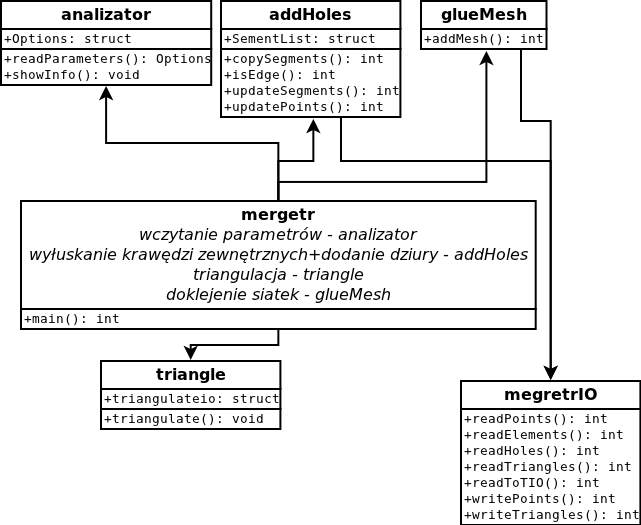
\includegraphics[scale=0.7]{img/diagram.png}
\caption{Diagram klas programu mergetr}
\end{figure}


\subsection{Struktura programu}

Program będzie się składał z następujących modułów:
\begin{enumerate}
\item Moduł przetwarzający wywołanie programu z linii komend (parser)
\item Moduł obsługujący wejście/wyjście z plików do struktur programu (i odwrotnie) \textit{Triangle} (mergetrIO)
\item Moduł zamieniający siatki na dziury w otoczce (addHoles)
\item Moduł triangulujący nową figurę (\textit{Triangle})
\item Moduł doklejający siatki początkowe do wygenerowanej (glueMesh)
\end{enumerate}

\subsection{Funkcjonalność poszczególnych modułów}
\begin{enumerate}

\item Moduł przetwarzający wywołanie programu z linii komend (parser)

\begin{itemize}
\item Za pomocą funkcji \textit{getopt} przetwarza tablicę char** argv
\item Wypełnia strukturę danych niezbędnymi danymi (nazwy plików, parametry \textit{Triangle})
\end{itemize}

\item Moduł wejścia/wyjścia plikow i struktur danych (mergetrIO)
\begin{itemize}
\item Czyta dane o wierzchołkach z pliku (czyta plik *.poly i *.node)
\item Czyta dane o trójkątach z pliku (czyta plik *.ele)
\item Czyta dane o dziurach z pliku (czyta plik *.poly)
\item Czyta dane o odcinkach z pliku (czyta plik *.poly)
\item Pisze dane o punktach do pliku (pisze plik *.node)
\item Pisze dane o trójkątach do pliku (pisze plik *.ele)
\end{itemize}

\item Moduł zamieniający siatki na dziury w otoczce (addHoles)

\begin{itemize}
\item Tworzy listę wszystkich krawędzi (zapamiętuje oba wierzchołki i informację, czy jest krawędzią zewnętrzną)
\item Tworzy listę punktów siatki (zapamiętuje numer w siatce, nowy numer w otoczce i informację, czy jest punktem zewnętrznym)
\item Zaznacza, które krawędzie i punkty są zewnętrze, a które nie
\item Kopiuje zewnętrzne punkty do otoczki
\item Kopiuje zewnętrzne odcinki do otoczki
\item Dodaje dziure w otoczce w miejscu siatki (środek ciężkości pierwszego trójkąta siatki)
\end{itemize}

\item Moduł triangulujący nową figurę (triangulation)
\begin{itemize}
\item Inicjuje struktury \textit{triangulateio}
\item Trianguluje zmodyfikowany wielokąt (po dodaniu dziur) za pomocą funkcji \textit{triangulate}
\end{itemize}

\item Moduł doklejający siatki początkowe do wygenerowanej (glueMesh)
\begin{itemize}
\item Kopiuje do striangulowanej otoczki wewnętrzne punkty siatki
\item Uaktualnia numery punktów w otoczce (ponieważ po triangulacji zmienia się porządek punktów)
\item Kopiuje trójkąty z siatki do otoczki według nowej numeracji
\item Usuwa dziurę stworzoną w miejscu siatki
\end{itemize}

\end{enumerate}

\subsection{Szczegółowy opis modułów - struktury danych i prototypy funkcji}

Każdy moduł składa się z pliku nagłówkowego, w którym znajdują się deklaracje struktur danych oraz funkcji wykorzystywanych w tym module oraz pliku z rozszerzeniem *.c zawierającym definicje funkcji. Całość jest połączona przez moduł sterujący - mergetr.c. Program \textit{Triangle} jest w programie użyty jako moduł do triangulacji wielokąta.
 
Oprócz modułów na program składa się plik \textit{makefile}, który umożliwia zbudowanie programu za pomocą narzędzia \textit{GNU Make}.

\begin{enumerate}
\item Przetwarzanie wywołania z linii komend (parser)

Do przechowywania parametrów wywołania służy struktura:

\begin{lstlisting}
typedef struct  
{
	char *input;             /* input file nameo */
	char *output;            /* output file name */
	char tr_opt[16];         /* Triangle options */
	int  args_start;         /* index of argv where arguments start */
} Options;
\end{lstlisting}

\begin{itemize}

\item Funkcja odczytująca opcje i argumenty z \textit{char **argv} za pomocą funkcji z biblioteki unistd \textit{getopt}, zwraca poprawnie wypełnioną strukturę. W przypadku, gdy nie zostały podane zostaną ustawione wartości domyślne.

\begin{lstlisting}
Options readParameters (int argc, char **argv);
\end{lstlisting}

\item W przypadku nie podania argumentów dla programu, podania niewystarczającej ich liczby lub podania błędnego argumentu dla opcji wyświetla informację o argumentach i dostępnych opcjach.
\begin{lstlisting}
void showInfo ();
\end{lstlisting}

\end{itemize}

\item Czytanie plików z danymi (megretrIO)

Moduł korzysta ze struktury \textit{triangulateio} (opisane w dokumentacji \textit{Triangle'a}) - zawierających wszystkie informacje o siatce.

\begin{itemize}

\item Funkcja wypełnia tablicę \textit{pointlist} z podanego pliku.
\begin{lstlisting}
int readPoints (FILE *in, struct triangulateio *x); 
\end{lstlisting}

\item Funkcja wypełnia tablicę \textit{pointargumentlist} z podanego pliku.
\begin{lstlisting}
int readSegments (FILE *in, struct triangulateio *x);
\end{lstlisting}

\item Funkcja wypełnia tablicę \textit{holelist} z podanego pliku.
\begin{lstlisting}
int readHoles (FILE *in, struct triangulateio *x);
\end{lstlisting}

\item Funkcja wypełnia tablicę \textit{trianglelist} z podanego pliku. 
\begin{lstlisting}
int readTriangles (FILE *in, struct triangulateio *x);
\end{lstlisting}

\item Zapisuje punkty z tablicy \textit{pointlist} do pliku
\begin{lstlisting}
int writePoints (FILE *out, struct triangulateio x); 
\end{lstlisting}

\item Zapisuje punkty z tablicy \textit{segmentlist} do pliku
\begin{lstlisting}
int writeSegments (FILE *out, struct triangulateio x);
\end{lstlisting}

\item Zapisuje trójkąty z tablicy \textit{trianglelist} do pliku
\begin{lstlisting}
int writeTriangles (FILE *out, struct triangulateio x); 
\end{lstlisting}

\item Zapisuje dziury z tablicy \textit{holelist} do pliku
\begin{lstlisting}
int writeHoles (FILE *out, struct triangulateio x); 
\end{lstlisting}
\end{itemize}

\item Zamiana siatek wejściowych na dziury (addHoles)

Moduł do wklejania siatek do otoczki wykorzystuje dwie własne struktury danych:

\begin{lstlisting}
typedef struct {
	int v1, v2; 
	int is_border; 
} EdgeList;
\end{lstlisting}
Lista krawędzi, numery węzłów krawędzi i parametr, czy jest zewnętrzna.

\begin{lstlisting}
typedef struct {
	int no_in_mesh; 		
	int no_in_otoczka;	
	int is_border;			
} PointList;
\end{lstlisting}
Lista punktów, numer punktu w siatce, numer w otoczce po wklejeniu i parametr, czy jest zewnętrzny.

\begin{itemize}
\item Funkcja tworzy listę krawędzi, zwraca tablicę typu EdgeList
\begin{lstlisting}
EdgeList *createEdgeList (struct triangulateio siatka);
\end{lstlisting} 

\item Funkcja sprawdza, które krawędzie należą tylko do jednego trójkąta i wpisuje wartość "1" do pola is border
\begin{lstlisting}
int markBndEdges (struct triangulateio siatka, EdgeList *t);
\end{lstlisting} 

\item Funkcja tworzy listę punktów, zwraca tablicę typu PointList
\begin{lstlisting}
PointList *makePointList (struct triangulateio otoczka, struct triangulateio siatka, EdgeList *t);
\end{lstlisting}

\item Dwie funkcje, które modyfikują struktury otoczki i dopisują punkty oraz krawędzie oznaczone jako zewnętrzne. Ostatnia funkcja dodaje dziurę w miejscu środka ciężkości pierwszego trójkąta siatki
\begin{lstlisting}
int updatePoints (struct triangulateio *otoczka, struct triangulateio siatka, EdgeList *t, PointList *p);

int updateSegments (struct triangulateio *otoczka, struct triangulateio siatka, EdgeList *t, PointList *p);

int updateHoles (struct triangulateio *otoczka, struct triangulateio siatka);
\end{lstlisting}

\end{itemize}

\item Triangulacja nowej siatki

\begin{itemize}
\item Funkcja (pochodząca z programu \textit{Triangle}) trianguluje obszar opisany w strukturze. Dostaje otoczkę z dodanymi dziurami i zwraca strukturę triangulateio z siatką trójkątną
\begin{lstlisting}
void triangulate(char *triswitches, struct triangulateio *in, struct triangulateio *out, struct triangulateio *vorout)
void triangulate(triswitches, in, out, vorout)
char *triswitches;
struct triangulateio *in;
struct triangulateio *out;
struct triangulateio *vorout;
\end{lstlisting}
\end{itemize}

\item Sklejenie siatek wejściowych z wynikową (glueMesh)

\begin{itemize}

\item Ponieważ podczas tworzenia listy krawędzi, krawędzie niezewnętrzne występują dwukrotnie funkcja oznacza odpowiednio tylko po jednej z każdej pary 
\begin{lstlisting}
int markNotBndEdges (struct triangulateio siatka, EdgeList *t);
\end{lstlisting}

\item Ponieważ po triangulacji nie ma pewności, że punkty pozostały w takiej samej kolejności jak przed tym procesem funkcja sprawdza nowe numery punktów (odległość maksymalnie o epsilon - zdefiniowany w programie) 
\begin{lstlisting}
int fixPointListNumbers (struct triangulateio *out, struct triangulateio *otoczka, PointList *p);
\end{lstlisting}

\item Dwie funkcje dodają do struktry punkty i trójkąty z siatki wejściowej. Na końcu zostaje usunięta dziura zrobiona w miejsce siatki
\begin{lstlisting}
int glueNotBndPoints (struct triangulateio *out, struct triangulateio siatka, PointList *p);

int glueInteriorTriangles (struct triangulateio *out, struct triangulateio siatka, PointList *p);

int removeHole (struct triangulateio *out);
\end{lstlisting}

\end{itemize}

\end{enumerate}

\section{Testy}

\subsection{Przygotowanie testów}
Kolejne moduły i dodane funkcjonalności były testowane na bierząco. Na potrzeby testowania ich stworzono zestaw plików testowych składający się z:
\begin{itemize}
\item 3 otoczek 
\item 5 siatek wejściowych 

Poniżej opisano 3 testy, która mogą być automatycznie wykonane przez wywołanie poleceń make - \textit{make test1, make test2, make test3}. Do oglądania wyników można wykorzystać polecenie \textit{make showme}.
\end{itemize}

\subsection{Przeprowadzone testy}

\subsubsection{Test 1}

Test przeprowadzono poprzez wywołanie programu o składni:
\begin{lstlisting}
./mtr -p test/O1 -a0.01 test/A.1 test/F.1
\end{lstlisting}

Poniżej przedstawiono wygląd otoczki i siatek składających się na test:

\begin{center}
	\begin{figure}[c]
	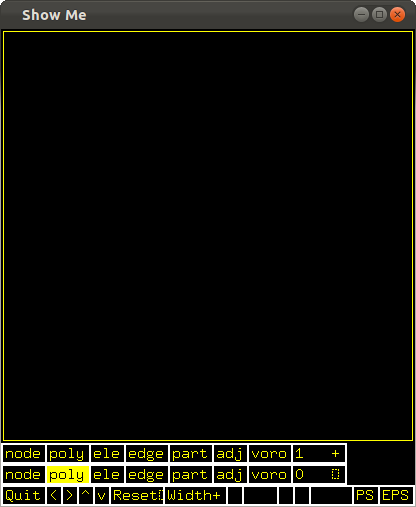
\includegraphics[scale=0.5]{img/O1.png}
	\caption{Otoczka - test/O1.poly}
\end{figure}

\begin{figure}[c]
	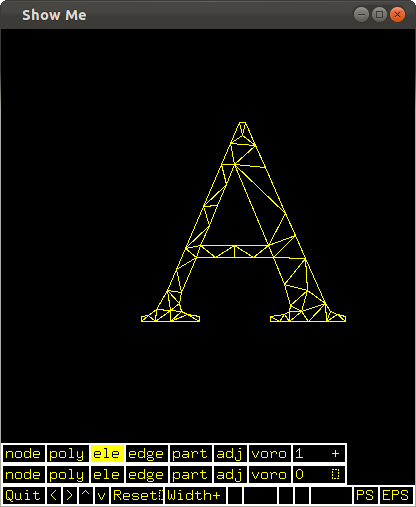
\includegraphics[scale=0.5]{img/A1.png}
	\caption{Siatka nr 1 - test/A.1}
\end{figure}

\begin{figure}[c]
	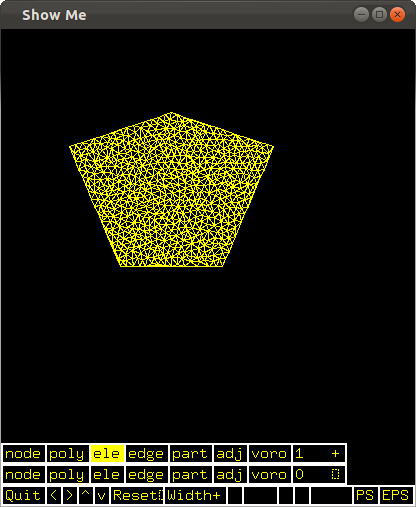
\includegraphics[scale=0.5]{img/F1.png}
	\caption{Siatka nr 2 - test/F.1}
\end{figure}

\end{center}

\subsubsection{Test2}
\end{document}
